%Version 3.1 December 2024
% See section 11 of the User Manual for version history
%
%%%%%%%%%%%%%%%%%%%%%%%%%%%%%%%%%%%%%%%%%%%%%%%%%%%%%%%%%%%%%%%%%%%%%%
%%                                                                 %%
%% Please do not use \input{...} to include other tex files.       %%
%% Submit your LaTeX manuscript as one .tex document.              %%
%%                                                                 %%
%% All additional figures and files should be attached             %%
%% separately and not embedded in the \TeX\ document itself.       %%
%%                                                                 %%
%%%%%%%%%%%%%%%%%%%%%%%%%%%%%%%%%%%%%%%%%%%%%%%%%%%%%%%%%%%%%%%%%%%%%

%%\documentclass[referee,sn-basic]{sn-jnl}% referee option is meant for double line spacing

%%=======================================================%%
%% to print line numbers in the margin use lineno option %%
%%=======================================================%%

%%\documentclass[lineno,pdflatex,sn-basic]{sn-jnl}% Basic Springer Nature Reference Style/Chemistry Reference Style

%%=========================================================================================%%
%% the documentclass is set to pdflatex as default. You can delete it if not appropriate.  %%
%%=========================================================================================%%

%%\documentclass[sn-basic]{sn-jnl}% Basic Springer Nature Reference Style/Chemistry Reference Style

%%Note: the following reference styles support Namedate and Numbered referencing. By default the style follows the most common style. To switch between the options you can add or remove �Numbered� in the optional parenthesis. 
%%The option is available for: sn-basic.bst, sn-chicago.bst%  
 
%%\documentclass[pdflatex,sn-nature]{sn-jnl}% Style for submissions to Nature Portfolio journals
%%\documentclass[pdflatex,sn-basic]{sn-jnl}% Basic Springer Nature Reference Style/Chemistry Reference Style
\documentclass[iicol,pdflatex,sn-basic,Numbered]{sn-jnl}% Basic Springer Nature Numbered Reference Style
%%\documentclass[pdflatex,sn-mathphys-ay]{sn-jnl}% Math and Physical Sciences Author Year Reference Style
%%\documentclass[pdflatex,sn-aps]{sn-jnl}% American Physical Society (APS) Reference Style
%%\documentclass[pdflatex,sn-vancouver-num]{sn-jnl}% Vancouver Numbered Reference Style
%%\documentclass[pdflatex,sn-vancouver-ay]{sn-jnl}% Vancouver Author Year Reference Style
%%\documentclass[pdflatex,sn-apa]{sn-jnl}% APA Reference Style
%%\documentclass[pdflatex,sn-chicago]{sn-jnl}% Chicago-based Humanities Reference Style

%%%% Standard Packages
%%<additional latex packages if required can be included here>

\usepackage{graphicx}%
\usepackage{multirow}%
\usepackage{amsmath,amssymb,amsfonts}%
\usepackage{amsthm}%
\usepackage{mathrsfs}%
\usepackage[title]{appendix}%
\usepackage{xcolor}%
\usepackage{textcomp}%
\usepackage{manyfoot}%
\usepackage{booktabs}%
\usepackage{algorithm}%
\usepackage{algorithmicx}%
\usepackage{algpseudocode}%
\usepackage{listings}%
\usepackage{array}%
\usepackage{tabularx}%
\usepackage{url}%
\hypersetup{hypertexnames=false}%
\newsavebox{\normalmetricbox}
\newcommand{\bestmetric}[1]{%
  \sbox{\normalmetricbox}{#1}%
  \resizebox{\wd\normalmetricbox}{\height}{\textbf{#1}}%
}
\newcommand{\metricdrop}[2]{#1\textcolor{red}{\ \(\downarrow\) #2\%}}
\newcommand{\metricgain}[2]{#1\textcolor{green!50!black}{\ \(\uparrow\) #2\%}}
\newcommand{\pgcell}[2]{\(\begin{aligned}p&=#1\\g&=#2\end{aligned}\)}
\newcommand{\pgcelllt}[1]{\(\begin{aligned}p&<10^{-4}\\g&=#1\end{aligned}\)}
%%%%

%%%%%=============================================================================%%%%
%%%%  Remarks: This template is provided to aid authors with the preparation
%%%%  of original research articles intended for submission to journals published 
%%%%  by Springer Nature. The guidance has been prepared in partnership with 
%%%%  production teams to conform to Springer Nature technical requirements. 
%%%%  Editorial and presentation requirements differ among journal portfolios and 
%%%%  research disciplines. You may find sections in this template are irrelevant 
%%%%  to your work and are empowered to omit any such section if allowed by the 
%%%%  journal you intend to submit to. The submission guidelines and policies 
%%%%  of the journal take precedence. A detailed User Manual is available in the 
%%%%  template package for technical guidance.
%%%%%=============================================================================%%%%

%% as per the requirement new theorem styles can be included as shown below
\theoremstyle{thmstyleone}%
\newtheorem{theorem}{Theorem}%  meant for continuous numbers
%%\newtheorem{theorem}{Theorem}[section]% meant for sectionwise numbers
%% optional argument [theorem] produces theorem numbering sequence instead of independent numbers for Proposition
\newtheorem{proposition}[theorem]{Proposition}% 
%%\newtheorem{proposition}{Proposition}% to get separate numbers for theorem and proposition etc.

\theoremstyle{thmstyletwo}%
\newtheorem{example}{Example}%
\newtheorem{remark}{Remark}%

\theoremstyle{thmstylethree}%
\newtheorem{definition}{Definition}%

\raggedbottom
%%\unnumbered% uncomment this for unnumbered level heads

\begin{document}

\title[Context-Aware Flight-Phase Anomaly Detection]{Context-Aware Flight-Phase Anomaly Detection via Cross-Perception Attention}

\author[1,2]{\fnm{Xiaodan} \sur{Wu}}

\author*[3]{\fnm{Yanan} \sur{Guo}}\email{guoyanan@mail.dhu.edu.cn}

\author[3]{\fnm{Kechen} \sur{Li}}

\author*[3]{\fnm{Zhong} \sur{Li}}\email{007lizhong@dhu.edu.cn}

\author[4]{\fnm{Xinzhong} \sur{Zhu}}

\author[1]{\fnm{Weiren} \sur{Zhu}}

\affil[1]{\orgdiv{School of Integrated Circuits}, \orgname{Shanghai Jiao Tong University}, \orgaddress{\city{Shanghai}, \postcode{200240}, \country{China}}}

\affil[2]{\orgname{Shanghai Aerospace Electronic Technology Institute}, \orgaddress{\city{Shanghai}, \postcode{201109}, \country{China}}}

\affil[3]{\orgdiv{School of Information and Intelligent Science}, \orgname{Donghua University}, \orgaddress{\city{Shanghai}, \postcode{201620}, \country{China}}}

\affil[4]{\orgdiv{Shanghai Institute of Satellite Engineering}, \orgaddress{\city{Shanghai}, \postcode{201109}, \country{China}}}

\abstract{With the rapid growth of civil aviation traffic, flight trajectory anomaly detection has become increasingly important for ensuring safety and efficiency. 
Although most existing models have achieved promising performance, they remain less suitable to capture trajectory deviations caused by dynamically changing regional conditions which jointly shape flight behaviors and are often weakly represented in the overall trajectory profile. 
To address this issue, we propose a Context-Aware Flight-Phase Anomaly Detection (CAFAD) method for fine-grained flight trajectory anomaly detection which identifies anomalies at the flight-phase level within specific airspace. 
We construct phase-specific context sets to provide reliable references for phase-level detection, each context set associated with a specific range of airspace and thereby serving as a localized normal reference. 
We then apply cross-perception attention between the target flight phase with its corresponding context-set memories to estimate phase-level anomaly scores, and aggregate the phase-level detection results to obtain the final trajectory-level anomaly decision. 
Experiments on real-world flight trajectory datasets show that CAFAD achieves the strongest F1 performance on the SJ-SA sub-datasets and remains competitive on UMN-UAV, supporting the value of fine-grained phase-level trajectory anomaly detection.}

\keywords{Aircraft trajectory, Anomaly detection, Aviation safety, Context-aware modeling, Cross-perception attention, Phase-level detection}

\maketitle

\section{Introduction}\label{sec:introduction}
With the rapid growth of civil aviation traffic, large-scale trajectory data provide an increasingly valuable basis for monitoring flight behaviors, identifying operational risks, and supporting proactive safety management~\cite{aerospace6110117}. 
Abnormal flight behaviors may indicate unstable maneuvers, unexpected route deviations, potential conflicts, airspace intrusions, traffic-management interventions, or abnormal responses to external disturbances~\cite{app12031295}. 
Therefore, developing detection models that can accurately identify abnormal flight trajectories has become an important research topic in both aviation safety and artificial intelligence~\cite{aerospace13030209,coelho2023analytics}.

Most existing flight trajectory anomaly detection models have achieved promising performance by modeling nominal trajectory patterns from historical data. 
Traditional approaches usually identify abnormal flights through clustering, density estimation, trajectory similarity analysis, Gaussian mixture models, or one-class classification~\cite{li2016gmm,diciccio2016detecting,olive:hal-02345597,9639966,olive2020significant,zhao2021incremental}. 
Recent deep learning methods further exploit recurrent neural networks, autoencoders, temporal convolutional networks, Transformer-based architectures, and prediction-based models to learn temporal dependencies and trajectory representations~\cite{doi:10.2514/1.I010941,chevrot2022cae,LUO2024103840,HUANG2025103478}. 
These models are effective for detecting obvious trajectory-level deviations . 
However, most of them still treat a complete trajectory as the main detection unit or evaluate the target trajectory mainly according to its own historical pattern, reconstruction error, or prediction inconsistency. 
Such a global or target-only formulation is often insufficient for fine-grained anomaly detection. 
Prior trajectory outlier studies~\cite{lee2008trajectory,yang2013trasmil,andrienko2018clustering} have shown that local abnormal portions of a long trajectory may be averaged out when the remaining portions follow normal patterns, rendering local anomalies statistically invisible within a global context.

Flight behaviors are highly context-dependent. 
In real-world operations, trajectory patterns are jointly shaped by the flight kinematic characteristics of aircraft itself and dynamically changing regional factors, including meteorological conditions, traffic flow, airspace constraints, and other environmental influences.
The localized spatio-temporal effects can cause the same deviation pattern to carry different meanings under different flight contexts.
For example, convective weather or thunderstorms may make a local detour normal~\cite{yang2024optimising}, rainy-season weather in terminal maneuvering areas may alter approach trajectories~\cite{chen2025impact}, and crosswinds or climate-induced performance degradation may affect takeoff and climb behavior~\cite{10.1145/3459104.3459109,williams2025quantifying,mcrae2021assessing}. 
Therefore, a model that is based on a global normal pattern may misclassify context-consistent group behaviors as anomalies~\cite{aerospace6110117,olive2020significant}, whereas a target-only model which detects anomalies of the target based on its own historical pattern may overlook abnormal behaviors that become apparent only through comparison with peer flights operating under similar conditions~\cite{chevrot2022cae,choi2023stochastic}.

This observation motivates a phase-level and context-aware perspective. 
A flight trajectory typically exhibits several operational phases~\cite{sun2017phaseidentification}, such as takeoff, cruise, and landing at a coarse level, while automatic phase identification can further partition these broad stages into finer motion-consistent segments. 
Therefore, it is more reasonable to evaluate the normality of a trajectory segment associated with a specific flight phase by comparing it with peer segments from other flights that are in the same local motion regime and operating under similar spatio-temporal conditions.
Compared with whole-trajectory detection, phase-level assessment relies on multiple matched context sets, enabling the model to identify localized contextual variations. 
In other words, the normality of a trajectory segment associated with the flight phase is evaluated conditionally with respect to phase-consistent and context-matched context sets which are highly relevant, rather than directly against a global trajectory distribution. 
In this way, weak but meaningful deviations can be amplified through cross-perception attention with relevant context sets, while normal group shifts caused by shared external factors can be better tolerated.

Another challenge lies in trajectory feature representation. 
Flight trajectories are irregularly sampled multivariate time series that typically include variables such as latitude, longitude, altitude, speed, heading, timestamp, etc~\cite{ahmed2026towards}.
The elapsed time between adjacent observations may vary due to reporting frequency, missing packets, and operational conditions. 
Generic sequence models based only on index order may therefore distort the true temporal spacing between observations~\cite{kreindler2016effects,li2020learning,kidger2020neuralcde,shukla2021mtnet,braun2022sampling}. 
Moreover, different trajectory variables carry distinct physical semantics. 
Spatial variables(latitude, longitude, altitude) describe where the aircraft moves, whereas kinematic variables(speed, heading) describe how it moves. 
Directly mixing these heterogeneous variables into a single homogeneous feature stream can blur their semantic roles and weaken discriminative representations for anomaly detection. 
Recent studies on multivariate time-series, structured-data, and flight trajectory representation learning have highlighted the importance of Transformer-based temporal modeling~\cite{zerveas2021transformer,xu2022anomalytransformer}, patch-based temporal representation~\cite{nie2023patchtst}, multi-scale temporal mixing~\cite{wang2024timemixer}, multi-temporal graph representation~\cite{guang2025mtpnet}, ensemble graph learning~\cite{guang2026ensnet}, and flight-specific trajectory representation~\cite{aerospace9020091,10877800,liu2025effective}.
However, these advances are still not fully aligned with context-aware anomaly detection in irregularly sampled flight trajectories.

To this end, we propose a context-aware flight-phase anomaly detection method. 
Instead of treating the whole trajectory as a single detection unit, CAFAD decomposes each trajectory into phase-level segments and evaluates each of them against matched context sets. 
Specifically, we construct phase-specific context sets by clustering automatically identified historical phase segments under similar spatio-temporal conditions. 
Then, a dual-branch time-aware transformer encoder is used to extract features of trajectory segments both in spatial and kinematic semantics while incorporating true elapsed-time information. 
By aggregating the features within each phase-specific context set, we obtain a context-set memory for that set.
Each context-set memory implicitly characterizes the dynamic regional context shared by flights traversing the corresponding airspace, thereby providing a localized normal reference for anomaly detection. 
Finally, we perform cross-perception attention between the features of the phase segments of the target trajectory and their corresponding context-set memories to estimate phase-level anomaly scores, and aggregate the phase-level detection results to obtain the final trajectory-level anomaly decision.
We conduct experiments on real-world flight trajectory datasets, and the results show that the proposed method achieves the strongest F1 performance on the SJ-SA sub-datasets while remaining competitive on UMN-UAV.

The main contributions of this paper are summarized as follows:
\begin{itemize}
    \item We reformulate flight trajectory anomaly detection as a fine-grained phase-level assessment problem. 
    Instead of directly judging the whole trajectory, the proposed framework detects anomalies at the flight-phase level and aggregates phase-level evidence for trajectory-level decision making.

    \item We introduce phase-specific context sets as localized normal references for context-aware anomaly detection.
    Rather than evaluating each phase segment in isolation, CAFAD organizes peer trajectory segments operating under similar spatio-temporal conditions into context sets and further summarizes them as context-set memories, allowing the model to characterize context-dependent normal flight behaviors and distinguish true anomalies from shared operational variations.

    \item We design a dual-branch time-aware transformer architecture to faithfully represent flight trajectory data. 
    By separately modeling spatial and kinematic variables while incorporating true elapsed-time information, the encoder preserves the heterogeneous semantics and temporal structure of irregularly sampled characteristics.

    \item Experiments on real-world flight trajectory datasets show that CAFAD achieves the strongest F1 performance on the SJ-SA sub-datasets while remaining competitive on UMN-UAV, supporting the value of phase-level contextual modeling for fine-grained trajectory anomaly detection.
\end{itemize}

The rest of this paper reviews related work, describes the proposed context-aware flight-phase anomaly detection method, reports experimental results, and discusses conclusions and future work.

\section{Related Work}\label{sec:related_work}

\subsection{Flight Trajectory Anomaly Detection}

Existing flight trajectory anomaly detection studies can be broadly divided into statistical/clustering-based methods and deep learning methods.
Statistical and clustering-based methods usually aim to discover nominal flight-operation patterns and then identify samples that deviate from these patterns.
Li et al.~\cite{li2016gmm} used Gaussian mixture models to characterize multiple normal flight-operation patterns, and Zhao et al.~\cite{zhao2021incremental} extended this idea with incremental updates for accumulating flight data. 
These methods provide interpretable references, but they are usually defined at a relatively coarse granularity.

Trajectory clustering has also been used to analyze historical aircraft trajectories.
Olive et al.~\cite{olive:hal-02345597,olive2020significant} combined trajectory clustering with anomaly detection to identify anomalous en-route trajectories, and subsequent studies further used clustering to analyze significant events and summarize common anomaly types in historical traffic data~\cite{aerospace13030209}. 
These studies show that clustering can organize common traffic patterns, but they still mainly focus on complete trajectories, traffic flows, or historical events rather than phase-level context sets.

More recent deep models have been introduced to improve temporal dependency modeling in flight trajectory and UAV trajectory anomaly detection.
Representative methods include contextual autoencoders, temporal convolutional networks, Transformer-based models, and prediction-based frameworks~\cite{chevrot2022cae,LUO2024103840,HUANG2025103478}.
These methods improve sequence representation for flight trajectories.
Most of them still use the whole trajectory or a long sequence as the main detection unit, which makes weak anomalies in local flight phases harder to highlight~\cite{lee2008trajectory,laxhammar2012online,yang2013trasmil}. 
They also mainly rely on reconstruction errors, prediction errors, or global normal patterns, with limited use of comparisons among flights under similar operational contexts.
As a result, localized and context-dependent deviations are not always easy to assess.

\subsection{Context-Aware and Phase-Aware Trajectory Modeling}

Beyond trajectory-level detectors, another line of work incorporates phase information or operational context into trajectory modeling.
Flight phase identification provides meaningful operational partitions because different flight phases correspond to different motion regimes and operational constraints~\cite{sun2017phaseidentification}. 
Sun et al.~\cite{sun2017phaseidentification} extracted flights from large-scale trajectory data and proposed a phase identification method for locating operational transitions, which provides a basis for phase-aware trajectory analysis. 
Arts et al.~\cite{arts2022trajectory} further combined trajectory segmentation with sequence classification to capture phase transitions and model flight dynamics.
These studies support phase-aware analysis, but they mainly stop at phase identification rather than phase-specific anomaly assessment.

Phase-aware modeling has also been explored in deep anomaly detection.
Chevrot et al.~\cite{chevrot2022cae} proposed a contextual autoencoder with multiple phase-specific decoders for multivariate time-series anomaly detection in air transportation. 
However, it mainly introduces phase awareness through reconstruction modules, without explicitly constructing phase-level context sets or comparing a target phase with flights under similar conditions.

Operational context is another important factor in flight trajectory modeling.
Context-aware aviation studies have incorporated external conditions or phase information into trajectory prediction, anomaly analysis, and operational risk assessment~\cite{aerospace9020091,app12031295,aerospace13030209,coelho2023analytics,choi2023stochastic}. 
Other studies also indicate that weather, traffic demand, terminal-area constraints, and dynamic airspace conditions can induce coherent trajectory variations among multiple flights operating under similar conditions~\cite{yang2024optimising,chen2025impact,sydorenko2025optimizing}.
These studies indicate that trajectory normality depends on the surrounding operational environment.
Most of them, however, treat context as auxiliary input or explanatory information rather than constructing matched context sets for anomaly scoring.

\subsection{Deep Representation Learning for Time-Series Anomaly Detection}

Deep representation learning provides important technical foundations for modeling complex flight trajectory sequences.
Recurrent networks and autoencoder-based models have been used to learn temporal representations and detect abnormal patterns from flight trajectory sequences~\cite{chevrot2022cae,LUO2024103840}. 
Temporal convolutional networks further capture local temporal dependencies through convolutional operations~\cite{HUANG2025103478}. 
Attention-based anomaly detection models capture temporal associations for sequence-level anomaly scoring~\cite{xu2022anomalytransformer}. 
Recent general time-series representation models, such as TimesNet~\cite{wu2023timesnet}, TSMixer~\cite{chen2023tsmixer}, and TimeMixer~\cite{wang2024timemixer}, also provide useful architectures for modeling complex temporal patterns.
Attention mechanisms further enhance sequence modeling by adaptively capturing long-range dependencies and important temporal associations~\cite{xu2022anomalytransformer}. 
For irregularly sampled time series, existing studies have also emphasized the importance of modeling actual elapsed time rather than relying only on ordinal positions~\cite{kreindler2016effects,li2020learning,kidger2020neuralcde,shukla2021mtnet,braun2022sampling}. 
These methods offer useful sequence modeling tools for flight trajectory data.

However, generic time-series anomaly detection models are usually designed for general sequential data rather than flight-specific anomaly detection.
They usually emphasize temporal dependencies within the target sequence, while giving limited attention to operational phase, peer behavior, and regional context.
Most of them also process all variables in a unified feature space, which only partially reflects the different roles of spatial and kinematic variables.
As a result, they do not fully address the context-conditioned and phase-dependent nature of flight trajectory anomalies.

\section{Methodology}\label{sec:methodology}

\subsection{Problem Definition \& Notation}

Given a labeled flight trajectory dataset $\mathcal{D} = \{(T_i, Y_i)\}_{i=1}^N$, each trajectory $T_i$ is a time-ordered set of observations $\{(\mathbf{x}_{i,t}, t_{i,t})\}_{t=1}^{L_i}$, and $Y_i \in \{0,1\}$ indicates whether the sample point is normal (0) or anomalous (1).
Each observation contains spatial and kinematic variables:
\begin{equation}
\mathbf{x}_{i,t} = (\phi_{i,t}, \lambda_{i,t}, h_{i,t}, h^{(p)}_{i,t}, v_{i,t}, \psi_{i,t})
\end{equation}
where $\phi$ and $\lambda$ denote longitude and latitude, $h$ and $h^{(p)}$ denote horizontal and pressure altitude, and $v$ and $\psi$ denote speed and heading.

We decompose each point into spatial and kinematic vectors as
\begin{equation}
\label{eq:decomposition}
\mathbf{s}_{i,t} = (\phi_{i,t}, \lambda_{i,t}, h_{i,t}, h^{(p)}_{i,t}), \quad \mathbf{k}_{i,t} = (v_{i,t}, \psi_{i,t}).
\end{equation}
This design follows the heterogeneous physical meanings of flight variables and provides a structured basis for subsequent phase-level cross-perception.

Flight trajectories typically consist of a small number of operational phases with distinct motion regimes. 
Only flights with similar local motion context are worth comparing with the target.
Comparing phase segments rather than complete trajectories therefore provides more matched samples for phase-level anomaly assessment.
To operationalize this idea, we split trajectories into automatically identified fine-grained phase segments and group them into phase-specific context sets to obtain more reliable context sets for phase-level comparison.
In this work, segmentation follows the automatic phase identification method of Sun et al.~\cite{sun2017phaseidentification}, which partitions each trajectory into a variable number of contiguous motion-consistent segments according to operational transitions along the trajectory. 
As a result, even within a broad operational stage, local regime changes can produce additional finer segments when their motion characteristics differ from the surrounding portions. 
Accordingly, each trajectory $T_i$ can be partitioned into $K_i$ contiguous phase segments.
We denote the $k$-th phase segment of trajectory $i$ as
\begin{equation}
T^{t',t''}_{i,k} \triangleq \{(\mathbf{x}_{i,\tau}, t_{i,\tau})\}_{\tau=t'}^{t''}.
\end{equation}
Here, $i$ is the trajectory index, $K_i$ denotes the number of phase segments of trajectory $i$, $k \in\{1,\ldots,K_i\}$ is the segment-order index, and the superscripts $(t',t'')$ are the start/end indices of this phase segment within the original trajectory.

Let $L_{i,k}$ denote the length of phase segment $T^{t',t''}_{i,k}$.
For mini-batch training, we pad each phase segment to a common maximum length
$T_{\max}=\max\{L_{i,k}\}$ and use a binary validity mask $\mathbf{m}_{i,k}\in\{0,1\}^{T_{\max}}$ to indicate real observations versus padded positions where 1 indicates a valid observation and 0 indicates padding.

For trajectory anomaly detection, each phase segment $T^{t',t''}_{i,k}$ is treated as a basic detection unit.
The model evaluates whether each segment is anomalous relative to its matched context sets, and the final trajectory decision is obtained by aggregating the phase-level results across the whole trajectory.
If all segments are judged normal, the trajectory is classified as normal; otherwise, it is classified as anomalous.

\subsection{The Overall Framework}

Fig.~\ref{fig:method_overview} summarizes the overall workflow of CAFAD.
The framework first decomposes each flight trajectory into automatically identified fine-grained phase segments so that anomaly assessment can be performed at a finer granularity than complete-trajectory classification.
For each target segment, peer segments operating under similar spatio-temporal conditions are grouped into context sets, which serve as localized normal references.
CAFAD then uses a dual-branch time-aware Transformer to encode the target segment and the segments in each matched context set while preserving the different semantics of spatial and kinematic variables.
The encoded peer segments are aggregated into context-set memories, and cross-perception attention compares the target phase representation with these memories to produce phase-level anomaly scores.
Finally, the phase-level scores are aggregated to obtain the trajectory-level anomaly decision.

\begin{figure*}[t]
\centering
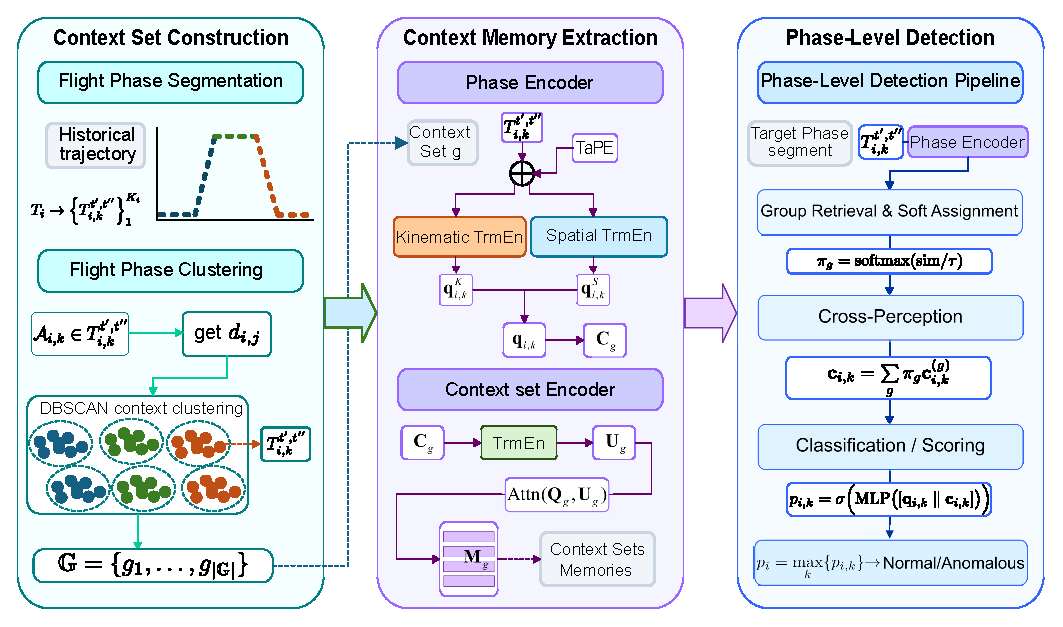
\includegraphics[width=\textwidth]{Fig1.eps}
\caption{Overview of CAFAD}
\label{fig:method_overview}
\end{figure*}

\subsection{Context Set Construction}
\label{sec:cohort_construction}

To enable reliable phase-level perception under heterogeneous environments and flight phases, we construct context sets that represent peer flight activities operating under similar spatio-temporal conditions.
In this stage, we use DBSCAN-based density clustering over \textbf{phase-specific segments} to build context sets.
This design enables group representations to capture shared running contexts while reducing contamination from heterogeneous motion regimes.

\subsubsection{Flight Phase Identification and Segmentation}

We segment each trajectory with the automatic phase identification method of Sun et al.~\cite{sun2017phaseidentification}.
This procedure identifies operational transitions from local motion characteristics and produces a variable number of contiguous, motion-consistent phase segments along each trajectory.
Consequently, a broad stage may be further divided into multiple finer segments when the underlying motion regime changes, such as a locally level-flight portion embedded within an overall descent.
In our implementation, these automatically identified fine-grained phase segments are used as the basic units for subsequent context set construction, thereby providing cleaner phase boundaries for downstream anomaly detection.

\subsubsection{Anchor Point Sampling}

The goal of context set construction is to identify shared operational contexts.
Clustering all points is computationally inefficient and biased toward long trajectories, so we adopt an anchor sampling strategy.
For each phase-specific segment $T^{t',t''}_{i,k}$, we sample a small set of anchor points $\mathcal{A}_{i,k}$ from its observations, with $|\mathcal{A}_{i,k}| \ll L_{i,k}$.
Each anchor point $a$ retains coarse contextual information $a=(t, x, y, \psi)$, where $(x,y)$ is a planar projection of $(\phi,\lambda)$ and $\psi$ is the heading.
Anchors can be obtained by uniform temporal sampling (e.g., one point per fixed time interval) or by selecting a small number of evenly spaced points across the segment duration so that each segment contributes comparably.

These anchors serve as lightweight representatives for phase-level context clustering.

\subsubsection{Spatio-temporal distance metric}

Because DBSCAN defines ``similar'' samples through an $\epsilon$-neighborhood, a key design choice is the distance measure: flight trajectories are sequences rather than single points, so the metric should reflect spatial, temporal, and dynamic similarity (e.g., similar shapes with slight sampling-time misalignment); accordingly, we define a normalized spatio-temporal distance between two anchor points $a_i=(t_i,x_i,y_i,\psi_i)$ and $a_j=(t_j,x_j,y_j,\psi_j)$ as
\begin{equation}
\label{eq:cohort_distance}
d(a_i,a_j)=
\sqrt{\left(\frac{\Delta t_{ij}}{\sigma_t}\right)^2+\left(\frac{\Delta s_{ij}}{\sigma_s}\right)^2+\left(\frac{\Delta\psi_{ij}}{\sigma_{\psi}}\right)^2},
\end{equation}
where
\begin{align}
\Delta t_{ij} &= |t_i-t_j|,\\
\Delta s_{ij} &= \sqrt{(x_i-x_j)^2+(y_i-y_j)^2},\\
\Delta\psi_{ij} &= \min\big(|\psi_i-\psi_j|,\, 2\pi-|\psi_i-\psi_j|\big),
\end{align}
and $(\sigma_t,\sigma_s,\sigma_{\psi})$ control the relative scales of temporal, spatial, and directional differences.

\subsubsection{Density-based Context Set Construction and Segment Assignment}

For each flight trajectory phase segment $T^{t',t''}_{i,k}$, we collect anchors and apply a density-based clustering method (DBSCAN) under $d(\cdot,\cdot)$.
Each resulting cluster corresponds to a spatio-temporally similar operational context (a context set), while anchors that do not belong to any dense region are treated as noise.

We map clusters back to phase segments by assigning a phase segment $T^{t',t''}_{i,k}$ to a context set when a sufficient fraction of its anchors $\mathcal{A}_{i,k}$ are assigned to the same DBSCAN cluster.
Segments whose anchors are mostly labeled as noise are retained and handled as low-support contexts during detection (e.g., by falling back to a coarser context set or by using multiple candidate context sets with soft assignment in Section~\ref{sec:segment_detection}), rather than being directly treated as anomalous. The output of this stage is a set of phase-consistent context sets $\mathbb{G}=\{g_1,\ldots,g_{|\mathbb{G}|}\}$.
Each context set $g\in\mathbb{G}$ is a set of phase segments.

\subsection{Context-Set Memory Encoding via Two-level Transformers}
\label{sec:group_memory_encoding}

We represent each context set as a set of learnable context-set memories extracted from historical segments within the same context set and phase.
Our encoding follows a two-level design: Level-1 encodes within-trajectory patterns, and Level-2 aggregates across trajectories to obtain context-set-level memories.

\subsubsection{Level-1: Intra-trajectory Dual-branch Time-aware Encoder}

Flight trajectories are described by heterogeneous spatial and kinematic variables that encode different physical aspects. As discussed in the Introduction, naively mixing such variables can introduce spurious correlations and incorrect dependencies driven by co-occurrence rather than physical causality.
To make this structure explicit, we decompose each point into spatial features $\mathbf{s}_{i,t} \in \mathbb{R}^4$ (longitude, latitude, horizontal altitude, pressure altitude) and kinematic features $\mathbf{k}_{i,t} \in \mathbb{R}^2$ (speed, heading), as defined in Equation~(\ref{eq:decomposition}).

Building on this decomposition, the proposed dual-branch time-aware encoder separately models the spatial (where) and kinematic (how) components of each trajectory segment, encouraging physically meaningful dependencies within each stream. Transformer encoders are well-suited for long, irregularly-sampled trajectories because self-attention captures long-range dependencies and enables efficient parallel computation. The dual-branch design allows each stream to specialize while reducing cross-stream interference; we then concatenate the branch-wise segment representations for downstream phase-level modeling.

\textbf{Spatial branch.} The spatial component is first embedded and processed through a Transformer encoder:
\begin{equation}
\mathbf{X}_{i,k}^S = \tilde{\mathbf{S}}_{i,k} \mathbf{W}_{emb}^S + \mathbf{b}_{emb}^S
\end{equation}
\begin{equation}
\mathbf{H}_{i,k}^S = \text{TrmEn}^S(\mathbf{X}_{i,k}^S + \mathrm{TaPE}(\Delta t), \mathbf{A}_{i,k})
\end{equation}
where $\tilde{\mathbf{S}}_{i,k} \in \mathbb{R}^{T_{\max} \times 4}$ is the padded spatial sequence for each $T^{t',t''}_{i,k}$, $\mathbf{W}_{emb}^S \in \mathbb{R}^{4 \times d_{model}}$ is the spatial embedding matrix, $\mathbf{b}_{emb}^S$ is the bias vector, $\text{TrmEn}^S$ denotes the spatial Transformer encoder, and $\mathbf{H}_{i,k}^S \in \mathbb{R}^{T_{\max} \times d_{model}}$ captures spatial trajectory patterns. The attention mask $\mathbf{A}_{i,k} \in \{0, -\infty\}^{T_{\max} \times T_{\max}}$ is constructed from $\mathbf{m}_{i,k}$ as:
\begin{equation}
\mathbf{A}_{i,k} = (\mathbf{1} - \mathbf{m}_{i,k}\,\mathbf{m}_{i,k}^{\top}) \odot (-\infty)
\end{equation}
The outer product creates an additive mask that assigns $-\infty$ to invalid attention scores, which effectively prevents attention to padded positions.

\textbf{Kinematic branch.} Similarly, the kinematic component is encoded through a separate branch:
\begin{equation}
\mathbf{X}_{i,k}^K = \tilde{\mathbf{K}}_{i,k} \mathbf{W}_{emb}^K + \mathbf{b}_{emb}^K
\end{equation}
\begin{equation}
\mathbf{H}_{i,k}^K = \text{TrmEn}^K(\mathbf{X}_{i,k}^K + \mathrm{TaPE}(\Delta t), \mathbf{A}_{i,k})
\end{equation}
where $\tilde{\mathbf{K}}_{i,k} \in \mathbb{R}^{T_{\max} \times 2}$ is the padded kinematic sequence, $\mathbf{W}_{emb}^K \in \mathbb{R}^{2 \times d_{model}}$ is the kinematic embedding matrix, $\mathbf{b}_{emb}^K$ is the bias vector, $\text{TrmEn}^K$ denotes the kinematic Transformer encoder, and $\mathbf{H}_{i,k}^K \in \mathbb{R}^{T_{\max} \times d_{model}}$ captures kinematic behavior patterns.

\textbf{Time-aware positional encoding.} Traditional positional encoding (e.g., in NLP) assumes uniform spacing and encodes ordinal positions (1st, 2nd, 3rd...), which fails to capture the physical time intervals crucial for flight dynamics.
To handle the irregular sampling nature of flight trajectory data, we employ time-aware positional encoding based on actual timestamps rather than sequence indices.

Given trajectory timestamps of a phase segment $T^{t',t''}_{i,k}$ with $\{t_{i,1}, t_{i,2}, \ldots, t_{i,L_{i,k}}\}$, we compute the relative time offset from the trajectory start:
\begin{equation}
\Delta t_{i,j} = t_{i,j} - t_{i,1}, \quad j = 1, 2, \ldots, L_{i,k}
\end{equation}

We then encode these relative time offsets using sinusoidal functions with different frequencies:
\begin{equation}
\mathrm{TaPE}(\Delta t)_{2\ell} = \sin\left(\frac{\Delta t}{10000^{2\ell/d_{model}}}\right)
\end{equation}
\begin{equation}
\mathrm{TaPE}(\Delta t)_{2\ell+1} = \cos\left(\frac{\Delta t}{10000^{2\ell/d_{model}}}\right)
\end{equation}
for $\ell = 0, 1, \ldots, d_{model}/2 - 1$, where $d_{model}$ is the model dimension.

Overall, TaPE encodes each observation by its true elapsed time, making temporal representations comparable across flights with different absolute start times and robust to non-uniform sampling intervals. The sinusoidal multi-scale design further supports capturing both short- and long-range temporal patterns in irregularly-sampled trajectories.

\textbf{Time-aware weighted pooling.} After branch-wise Transformer encoding, the hidden states $\mathbf{H}_{i,k}^S$ and $\mathbf{H}_{i,k}^K$ still retain point-level representations aligned with irregular timestamps.
To obtain a fixed-dimensional representation while explicitly accounting for non-uniform sampling intervals, we adopt a time-aware weighted pooling strategy for each branch.

Specifically, let $\mathbf{H}_{i,k,j}^S$ and $\mathbf{H}_{i,k,j}^K$ denote the spatial and kinematic hidden states at time step $j$, and let $\Delta t_{i,j} = t_{i,j} - t_{i,j-1}$ be the elapsed time between two consecutive valid observations (with $\Delta t_{i,1}$ defined as zero or a small constant).
We compute branch-wise pooled representations as:
\begin{equation}
\label{eq:segment_pool}
\begin{aligned}
\mathbf{q}_{i,k}^S &=
\frac{\sum\limits_{j=1}^{L_{i,k}} \Delta t_{i,j}\,\mathbf{H}_{i,k,j}^S}
{\sum\limits_{j=1}^{L_{i,k}} \Delta t_{i,j}},\\
\mathbf{q}_{i,k}^K &=
\frac{\sum\limits_{j=1}^{L_{i,k}} \Delta t_{i,j}\,\mathbf{H}_{i,k,j}^K}
{\sum\limits_{j=1}^{L_{i,k}} \Delta t_{i,j}}.
\end{aligned}
\end{equation}
where $\mathbf{q}_{i,k}^S \in \mathbb{R}^{d_{model}}$ and $\mathbf{q}_{i,k}^K \in \mathbb{R}^{d_{model}}$ denote the time-aware pooled spatial and kinematic representations of the phase segment $T^{t',t''}_{i,k}$, respectively.

This pooling operation assigns larger weights to trajectory points that persist over longer physical time intervals, preventing densely sampled regions from dominating the representation.
Compared with mean or max pooling, time-aware weighted pooling better reflects the true temporal contribution of each observation and is particularly suitable for flight data with variable reporting rates and missing points.

Finally, the phase-level trajectory representation is obtained by concatenating the pooled outputs of the two branches:
\begin{equation}
\mathbf{q}_{i,k} = \big[\,\mathbf{q}_{i,k}^S \,\|\, \mathbf{q}_{i,k}^K\,\big],
\end{equation}
which preserves the semantic separation between spatial structure and kinematic dynamics while providing a compact representation for downstream context-aware modeling and anomaly detection.

\subsubsection{Level-2: Inter-trajectory Context Encoder}

After obtaining phase-level representations from the intra-trajectory dual-branch encoder, we further model interactions among multiple trajectories operating under the same spatio-temporal context. This is achieved through an inter-trajectory Transformer, which aggregates peer trajectory information within each context set and constructs a context-set-level memory.

\textbf{Context-set token construction.}
For a given context set $g$, we collect the phase-level embeddings of all trajectory segments assigned to this context set $\mathbf{C}_g$.
Each token encapsulates the spatial structure and kinematic dynamics of an individual trajectory segment within a specific flight phase.

\textbf{Inter-trajectory contextual encoding.}
To capture higher-order interactions and shared behavioral patterns among peer trajectories, we feed $\mathbf{C}_g$ into a context-set Transformer encoder:
\begin{equation}
\mathbf{U}_g = \mathrm{Trm}(\mathbf{C}_g)
\in \mathbb{R}^{|g| \times 2d_{model}},
\end{equation}
where $\mathrm{Trm}(\cdot)$ denotes a standard Transformer encoder operating across the trajectory dimension. 
Through self-attention, this module enables each trajectory token to attend to other peer trajectories within the same context set, thereby encoding contextual dependencies induced by shared environmental conditions, airspace constraints, and traffic interactions.
Unlike trajectory-level encoders that focus on temporal dependencies, the inter-trajectory Transformer models population-level correlations across multiple flights, allowing the network to capture coherent group behaviors such as coordinated detours, common climb or descent profiles, and traffic-induced flow patterns.

\textbf{Context-set memory construction via attention pooling.}
Since the number of trajectories $|g|$ varies across context sets, we introduce a fixed-size context-set memory to summarize group-level information. Specifically, we employ $m$ learnable query vectors, where $m$ denotes the number of context-set memory slots,
\begin{equation}
\mathbf{Q}_g \in \mathbb{R}^{m \times 2d_{model}},
\end{equation}
and perform attention-based pooling over the encoded context-set representations:
\begin{equation}
\label{eq:inter_traj}
\mathbf{M}_g = \mathrm{Attn}(\mathbf{Q}_g, \mathbf{U}_g, \mathbf{U}_g)
\in \mathbb{R}^{m \times 2d_{model}}.
\end{equation}

Here, $\mathrm{Attn}(\cdot)$ denotes scaled dot-product attention, where $\mathbf{Q}_g$ acts as queries and $\mathbf{U}_g$ serves as both keys and values. Each row of $\mathbf{M}_g$ aggregates information from multiple trajectories in the context set, enabling the memory to capture diverse yet representative phase-level behavioral modes.

The resulting memory matrix $\mathbf{M}_g$ can be interpreted as a context-set memory representation that characterizes typical flight behaviors under the current operational context and flight phase. Importantly, this memory provides a flexible, multi-slot representation that encodes common patterns and sub-modes emerging from peer trajectories, such as environment-driven deviations or traffic-induced maneuvers.
By using this context-set-level memory as context for subsequent anomaly assessment, the model can distinguish true abnormal behaviors from context-driven deviations that are shared by multiple flights, thereby improving robustness and reducing false alarms.

\subsection{Phase-Level Detection for Trajectory Anomaly Assessment}
\label{sec:segment_detection}
Given a target phase segment $T^{t',t''}_{i,k}$, we encode the segment into a phase-level representation and then compute a context-aware embedding by matching it against the retrieved context-set memories.


\subsubsection{Segment Encoder}

We use the Level-1 encoder (shared weights) to obtain branch-wise hidden states and a pooled phase embedding $\mathbf{q}_{i,k}$ as in Eq.~(\ref{eq:segment_pool}), with the input sequence taken as the phase segment $T^{t',t''}_{i,k}$.


\subsubsection{Group Retrieval and Soft Assignment}

Following Section~\ref{sec:cohort_construction}, we first determine the assigned context-set index $g_{i,k}$ for segment $T^{t',t''}_{i,k}$.
We then retrieve the corresponding context-set memory $\mathbf{M}_{g_{i,k}}$ obtained by Eq.~(\ref{eq:inter_traj}).
For simplicity, we denote this retrieved memory by $\mathbf{M}_{i,k}$.
To be robust to context-set ambiguity (e.g., boundary cases across nearby context sets or phases), we optionally retrieve multiple candidate context sets and compute a soft assignment weight for each candidate based on similarity:
\begin{equation}
\label{eq:soft_assign}
\pi_g = \frac{\exp(\text{sim}(\mathbf{q}_{i,k}, \bar{\mathbf{m}}_g)/\tau)}{\sum\limits_{g'\in\mathcal{C}(i,k)} \exp(\text{sim}(\mathbf{q}_{i,k}, \bar{\mathbf{m}}_{g'})/\tau)},
\end{equation}
where $\mathcal{C}(i,k)$ is the set of candidate context sets, $\bar{\mathbf{m}}_g$ is a pooled summary of group memories (e.g., mean over slots), and $\tau$ is a temperature.

\subsubsection{Cross-Perception Attention}

We compute cross-attention from the individual phase embedding to the retrieved context-set memories:
\begin{equation}
\label{eq:cross_perception}
\mathbf{c}_{i,k} = \text{CrossAttn}(\mathbf{q}_{i,k}, \mathbf{M}_{i,k}),
\end{equation}
where $\mathbf{q}_{i,k}$ acts as the query and the memory slots act as keys/values.
If multiple candidate context sets are retrieved, their contexts are combined by the assignment weights $\pi_g$:
The weight $\pi_g$ enables uncertainty-aware context fusion, reducing sensitivity to hard retrieval errors and improving robustness for boundary segments.
\begin{equation}
\mathbf{c}_{i,k} = \sum_{g\in\mathcal{C}(i,k)} \pi_g\, \text{CrossAttn}(\mathbf{q}_{i,k}, \mathbf{M}_{g}).
\end{equation}

\subsubsection{Classification / Scoring}

Finally, we concatenate the phase and context representations and predict an anomaly probability for the target segment:
\begin{equation}
\label{eq:segment_score}
s_{i,k} = \text{MLP}([\mathbf{q}_{i,k} \| \mathbf{c}_{i,k}]), \quad p_{i,k} = \sigma(s_{i,k}).
\end{equation}
The concatenated vector combines the local phase representation and the context-aware evidence, so the classifier can assess a segment from both its intrinsic behavior and its peer-context consistency.
The MLP produces an unnormalized anomaly score, and the sigmoid function converts it into the final anomaly probability.
The final trajectory decision is then obtained by aggregating the phase-level probabilities of all phase segments in the trajectory, and the trajectory is judged anomalous if at least one segment is detected as anomalous.

\subsection{Loss Function}

We train the model with a trajectory-level focal loss~\cite{lin2017focal} applied to segment-aggregated predictions.
For each trajectory, we first aggregate the segment probabilities into a trajectory-level probability by
\begin{equation}
\label{eq:traj_agg}
p_i = \max_{1 \le k \le K_i} p_{i,k}.
\end{equation}
The loss is then defined as
\begin{equation}
\label{eq:focal_loss}
\begin{aligned}
\mathcal{L}_f = -\frac{1}{N} \sum_i \Bigl[
&\alpha\,Y_i(1-p_i)^{\gamma}\log p_i\\
&+ (1-Y_i)p_i^{\gamma}\log(1-p_i)
\Bigr],
\end{aligned}
\end{equation}
where $\alpha$ is a class-balancing weight and $\gamma$ is the focusing parameter.
This objective encourages the model to assign a high anomaly score to a trajectory whenever one of its phase segments exhibits behavior inconsistent with the matched context-set memories.

\subsection{Complexity Analyses}
We briefly analyze the computational complexity of the main modules in CAFAD.
For a phase segment of length $T_{\max}$, one Level-1 Transformer layer has the standard self-attention complexity $\mathcal{O}(T_{\max}^{2}d_{model})$.
For a context set $g$ with $|g|$ segments, one Level-2 inter-trajectory Transformer layer has complexity $\mathcal{O}(|g|^{2}d_{model})$.
In phase-level detection, soft assignment over candidate context sets has complexity linear in $|\mathcal{C}(i,k)|$, while cross-perception over $m$ memory slots is linear in $m$ for each target phase.
The trajectory-level aggregation in Eq.~(\ref{eq:traj_agg}) is linear in the number of phase segments.
The DBSCAN-based context-set construction is performed offline, and its cost depends on the number of sampled anchors.
Therefore, the dominant online inference cost is primarily from Level-1/Level-2 attention and cross-perception over retrieved memories.

\section{PERFORMANCE EVALUATION}\label{sec:performance_evaluation}
In this section, we present a comprehensive evaluation of the proposed anomaly detection model on real-world flight trajectory datasets.
The section is organized as follows.
The experimental settings subsection introduces the datasets, evaluation metrics, baseline methods, and implementation settings.
The following subsections report the main results, ablation study, parameter sensitivity analysis, and visualization analysis.

\subsection{Experimental Settings}

\subsubsection{Dataset Description}
\label{sec:dataset}

We evaluate CAFAD on two real-world flight trajectory datasets collected from different regions and operating environments, namely SJ-SA and UMN-UAV\cite{umn_uav_dataset}.
Their basic characteristics are summarized as follows.

\begin{itemize}
\item \textbf{SJ-SA}: This dataset was jointly collected by Shanghai Jiao Tong University and Shanghai Aerospace Electronic Technology Institute.
It contains five sub-datasets corresponding to flight trajectory data recorded from May to September in 2024.
The data were continuously received and recorded by ground-deployed high-performance surveillance and positioning receivers.
The dataset covers multiple flight phases, including takeoff, landing, and cruise.
The SJ-SA data used in this study are publicly available at \url{https://github.com/cydhu/data/tree/master}.
For each flight, complete state information at each timestamp, such as longitude, latitude, altitude, and speed, is recorded as the reference ground truth.

\item \textbf{UMN-UAV}: This dataset was collected and provided by the UAV Laboratory at the University of Minnesota, containing telemetry records from 342 flight missions conducted by small fixed-wing unmanned aerial platforms at an airport test site.
The missions were conducted in a spatially confined low-altitude test area spanning only a few kilometers, rather than across broad civil-aviation routes.
The data includes timestamped position and kinematic observations for each mission, together with annotations of aircraft type and performed maneuvers such as doublets and waypoint tracking.
\end{itemize}

For both datasets, trajectories are processed following the phase-specific segmentation strategy described in Section~\ref{sec:cohort_construction}.
The resulting phase segments are padded to a common maximum length $T_{\max}$, and validity masks are used to distinguish real observations from padded positions.
For inter-trajectory context-set memory encoding, the number of context-set memory slots is set to $m = 8$ as a practical trade-off between representational coverage and model complexity.


\subsubsection{Evaluation Metrics}
\label{sec:metrics}

We evaluate anomaly detection performance using four standard classification metrics: Accuracy (Acc), Precision (Pre), Recall, and F1.
All four metrics follow their standard definitions in classification evaluation~\cite{powers2020evaluation}.
Given the class imbalance inherent to anomaly detection, F1 serves as the primary indicator, while Recall reflects the model's sensitivity to anomalous trajectories.


\subsubsection{Baseline Methods}

We compare CAFAD against six baseline methods from classical long short-term memory to several recent state-of-the-art time-series models as follows:
\begin{itemize}
\item \textbf{TimesNet}~\cite{wu2023timesnet}: A temporal 2D-variation model that transforms 1D time series into 2D space for multi-period analysis via 2D convolution.
\item \textbf{TimeMixer}~\cite{wang2024timemixer}: A decomposable multiscale mixing architecture that disentangles seasonal and trend components for hierarchical feature aggregation.
\item \textbf{TSMixer}~\cite{chen2023tsmixer}: An MLP-Mixer-based model that applies alternating time-mixing and channel-mixing operations for multivariate time-series modeling.
\item \textbf{1D CNN-LSTM}~\cite{yang2024data}: A hybrid baseline that combines temporal convolution with recurrent sequence modeling.
\item \textbf{CTranATD}~\cite{Han2025CNNTransformerBA}: A stronger deep anomaly detection baseline included for broader comparison.
\end{itemize}
Ablation variants of our method are reported separately in Section~\ref{sec:ablation}.

\subsubsection{Implementation Settings}

\begin{table}[t]
  \centering
  \setlength{\tabcolsep}{2pt}
  \renewcommand{\arraystretch}{1.05}
  \caption{Hyperparameter settings for the proposed method}
  \label{tab:hyperparameters}
  \tablebodyfont
  \begin{tabularx}{\columnwidth}{@{}l>{\raggedright\arraybackslash}Xl@{}}
    \toprule
    Parameter & Description & Value \\
    \midrule
    $E$ & Max number of training epochs & 100 \\
    $B$ & Batch size & 64 \\
    $P$ & Dropout rate & 0.3 \\
    $L_m$ & Peak learning rate & $1 \times 10^{-4}$ \\
    $\omega_d$ & Weight decay coefficient & $1 \times 10^{-5}$ \\
    $N_p$ & Early stopping patience & 20 \\
    $N_H$ & Number of attention heads & 8 \\
    $N_E$ & Number of Transformer encoder layers & 6 \\
    $d_{model}$ & Transformer hidden dimension & 512 \\
    $N_f$ & Transformer feed-forward network dimension & 2048 \\
    $m$ & Number of context-set memory slots & 8 \\
    $\tau$ & Soft-assignment temperature & 1.0 \\
    $\sigma_t$ & Temporal scale in spatio-temporal distance & 10 \\
    $\sigma_s$ & Spatial scale in spatio-temporal distance & 10000 \\
    $\sigma_{\psi}$ & Heading scale in spatio-temporal distance & 3.14159 \\
    $\alpha$ & Weighting factor in focal loss & 0.25 \\
    $\gamma$ & Focusing parameter in focal loss & 2.0 \\
    \bottomrule
  \end{tabularx}
\end{table}
We implement the proposed context-aware flight-phase anomaly detection model in shared regional airspace and all baseline methods in Python~3.9.23, using NumPy~1.26.4, PyTorch~2.8.0, scikit-learn~1.6.1, and CUDA~12.8.
All experiments are conducted on a server equipped with an Intel(R) Xeon(R) Gold 6330 CPU @ 2.00GHz and an NVIDIA GeForce RTX 5090 GPU.
The GPU is equipped with 36\,GB of memory, and the server runs on Ubuntu~24.04.3 LTS.
We optimize the model parameters using the AdamW optimizer, train for at most 100 epochs, and set the early stopping patience to 20.
The hyperparameter settings used in our model are listed in Table~\ref{tab:hyperparameters}.
In each experiment, the dataset is split into 70\%, 15\%, and 15\% for training, validation, and testing, respectively.
To prevent data leakage caused by temporal correlation, the dataset partition is performed at the flight-trajectory level, ensuring that the same flight trajectory does not appear simultaneously in both the training set and the test set.
All experiments are repeated five times using random seeds 42, 142, 242, 342, and 442.

\subsection{Main Results}

Table~\ref{tab:main_results} reports the anomaly detection performance of CAFAD and six baseline methods across all six datasets.
All results are averaged over five independent runs with different random seeds and are presented as mean~$\pm$~standard deviation.
For each dataset and metric, the best result among all methods is highlighted in bold.

\begin{table*}[!t]
\centering
\caption{Anomaly detection performance comparison on the six flight trajectory datasets}
\label{tab:main_results}
\setlength{\tabcolsep}{1.5pt}
\renewcommand{\arraystretch}{0.95}
\footnotesize
\begin{tabularx}{\linewidth}{@{}ll*{7}{>{\centering\arraybackslash}X}@{}}
\toprule
\multirow{2}{*}{Dataset} & \multirow{2}{*}{Metric} & \multicolumn{7}{c}{Methods} \\
\cmidrule(lr){3-9}
& & TimesNet & TimeMixer & TSMixer & LSTM & \resizebox{\linewidth}{!}{1D CNN-LSTM} & CTranATD & Ours \\
\midrule
\multirow{4}{*}{SJ-SA-D1}
& Acc    & 0.8330$\pm$0.0689 & 0.8250$\pm$0.0700 & 0.8350$\pm$0.0644 & 0.8573$\pm$0.0178 & 0.8717$\pm$0.0285 & 0.8924$\pm$0.0115 & \bestmetric{0.9294$\pm$0.0050} \\
& Pre    & 0.8725$\pm$0.0248 & 0.8650$\pm$0.0204 & 0.8708$\pm$0.0314 & 0.8118$\pm$0.0053 & 0.9131$\pm$0.0100 & 0.8996$\pm$0.0185 & \bestmetric{0.9510$\pm$0.0157} \\
& Recall & 0.8192$\pm$0.0628 & 0.8112$\pm$0.0680 & 0.8162$\pm$0.0655 & 0.7920$\pm$0.0053 & 0.8089$\pm$0.0146 & 0.8621$\pm$0.0258 & \bestmetric{0.9057$\pm$0.0079} \\
& F1     & 0.8577$\pm$0.0154 & 0.8504$\pm$0.0154 & 0.8561$\pm$0.0186 & 0.8018$\pm$0.0053 & 0.8505$\pm$0.0195 & 0.8804$\pm$0.0223 & \bestmetric{0.9277$\pm$0.0058} \\
\midrule
\multirow{4}{*}{SJ-SA-D2}
& Acc    & 0.7098$\pm$0.0083 & 0.7012$\pm$0.0060 & 0.6931$\pm$0.0141 & 0.8789$\pm$0.0067 & 0.9019$\pm$0.0022 & \bestmetric{0.9111$\pm$0.0014} & 0.9019$\pm$0.0087 \\
& Pre    & 0.8289$\pm$0.0087 & 0.8282$\pm$0.0095 & 0.8276$\pm$0.0087 & 0.8348$\pm$0.0078 & 0.9148$\pm$0.0051 & 0.9192$\pm$0.0056 & \bestmetric{0.9657$\pm$0.0035} \\
& Recall & 0.7107$\pm$0.0069 & 0.6917$\pm$0.0027 & 0.6874$\pm$0.0124 & 0.7386$\pm$0.0035 & 0.7440$\pm$0.0089 & 0.7642$\pm$0.0130 & \bestmetric{0.8597$\pm$0.0102} \\
& F1     & 0.7652$\pm$0.0022 & 0.7538$\pm$0.0055 & 0.7510$\pm$0.0100 & 0.7838$\pm$0.0027 & 0.8206$\pm$0.0062 & 0.8345$\pm$0.0064 & \bestmetric{0.9096$\pm$0.0070} \\
\midrule
\multirow{4}{*}{SJ-SA-D3}
& Acc    & 0.7058$\pm$0.0126 & 0.7229$\pm$0.0091 & 0.7028$\pm$0.0111 & 0.8831$\pm$0.0035 & 0.9140$\pm$0.0037 & \bestmetric{0.9220$\pm$0.0046} & 0.9010$\pm$0.0034 \\
& Pre    & 0.8570$\pm$0.0039 & 0.8125$\pm$0.0073 & 0.8212$\pm$0.0112 & 0.8370$\pm$0.0043 & 0.9308$\pm$0.0049 & 0.9202$\pm$0.0073 & \bestmetric{0.9611$\pm$0.0045} \\
& Recall & 0.6832$\pm$0.0076 & 0.6731$\pm$0.0053 & 0.6894$\pm$0.0078 & 0.7608$\pm$0.0060 & 0.7710$\pm$0.0051 & 0.7942$\pm$0.0065 & \bestmetric{0.8372$\pm$0.0089} \\
& F1     & 0.7603$\pm$0.0060 & 0.7363$\pm$0.0043 & 0.7494$\pm$0.0054 & 0.7971$\pm$0.0043 & 0.8433$\pm$0.0018 & 0.8526$\pm$0.0027 & \bestmetric{0.8949$\pm$0.0064} \\
\midrule
\multirow{4}{*}{SJ-SA-D4}
& Acc    & 0.7332$\pm$0.0038 & 0.7219$\pm$0.0069 & 0.7271$\pm$0.0054 & 0.8800$\pm$0.0053 & \bestmetric{0.9193$\pm$0.0063} & 0.9149$\pm$0.0071 & 0.9132$\pm$0.0069 \\
& Pre    & 0.8404$\pm$0.0020 & 0.8433$\pm$0.0015 & 0.8432$\pm$0.0062 & 0.8348$\pm$0.0108 & 0.9385$\pm$0.0046 & 0.9471$\pm$0.0078 & \bestmetric{0.9782$\pm$0.0035} \\
& Recall & 0.7122$\pm$0.0135 & 0.7054$\pm$0.0049 & 0.7042$\pm$0.0044 & 0.7417$\pm$0.0081 & 0.7997$\pm$0.0059 & \bestmetric{0.8894$\pm$0.0040} & 0.8881$\pm$0.0077 \\
& F1     & 0.7710$\pm$0.0078 & 0.7682$\pm$0.0024 & 0.7674$\pm$0.0042 & 0.7854$\pm$0.0030 & 0.8635$\pm$0.0041 & 0.9173$\pm$0.0021 & \bestmetric{0.9310$\pm$0.0046} \\
\midrule
\multirow{4}{*}{SJ-SA-D5}
& Acc    & 0.7496$\pm$0.0109 & 0.7174$\pm$0.0177 & 0.7206$\pm$0.0108 & 0.7860$\pm$0.0019 & \bestmetric{0.9127$\pm$0.0058} & 0.9117$\pm$0.0084 & 0.8929$\pm$0.0060 \\
& Pre    & 0.8484$\pm$0.0037 & 0.7990$\pm$0.0070 & 0.8334$\pm$0.0083 & 0.7836$\pm$0.0077 & 0.9087$\pm$0.0030 & 0.9391$\pm$0.0060 & \bestmetric{0.9480$\pm$0.0069} \\
& Recall & 0.7232$\pm$0.0061 & 0.7037$\pm$0.0130 & 0.7158$\pm$0.0047 & 0.8004$\pm$0.0073 & 0.7875$\pm$0.0062 & 0.7807$\pm$0.0036 & \bestmetric{0.8620$\pm$0.0063} \\
& F1     & 0.7808$\pm$0.0041 & 0.7483$\pm$0.0095 & 0.7701$\pm$0.0046 & 0.7919$\pm$0.0031 & 0.8438$\pm$0.0042 & 0.8526$\pm$0.0043 & \bestmetric{0.9029$\pm$0.0016} \\
\midrule
\multirow{4}{*}{UMN-UAV}
& Acc    & 0.7310$\pm$0.0059 & 0.7182$\pm$0.0096 & 0.7074$\pm$0.0056 & \bestmetric{0.9854$\pm$0.0040} & 0.9850$\pm$0.0042 & 0.9685$\pm$0.0034 & 0.8883$\pm$0.0038 \\
& Pre    & 0.6995$\pm$0.0092 & 0.8348$\pm$0.0063 & 0.8294$\pm$0.0041 & 0.8707$\pm$0.0033 & \bestmetric{0.9615$\pm$0.0041} & 0.8014$\pm$0.0039 & 0.9336$\pm$0.0022 \\
& Recall & 0.6288$\pm$0.0087 & 0.7051$\pm$0.0037 & 0.6839$\pm$0.0042 & 0.7799$\pm$0.0098 & \bestmetric{0.8635$\pm$0.0060} & 0.5242$\pm$0.0092 & 0.8416$\pm$0.0096 \\
& F1     & 0.6622$\pm$0.0043 & 0.7644$\pm$0.0044 & 0.7497$\pm$0.0031 & 0.8228$\pm$0.0062 & \bestmetric{0.9098$\pm$0.0034} & 0.6338$\pm$0.0074 & 0.8852$\pm$0.0058 \\
\bottomrule
\end{tabularx}
\end{table*}

Across the five SJ-SA sub-datasets, CAFAD achieves the highest F1 and Precision, with F1 ranging from 0.8949 to 0.9310 and exceeding the strongest baseline by 1.37\%--7.51\%.
This consistent F1 and Precision advantage indicates that phase-specific context modeling helps CAFAD maintain a favorable balance between anomaly sensitivity and false-alarm control under monthly variations in flight operations.
The 95\% confidence intervals in Table~\ref{tab:appendix_f1_ci} show that CAFAD has clearly higher estimated F1 performance than all baselines on D1--D5.
The paired $t$-test $p$-values and Hedges' $g$ values in Table~\ref{tab:appendix_sig} show that the F1 advantage is statistically reliable against all six baselines on D1--D5, with large positive effect sizes in all comparisons.
The main exceptions concern Accuracy and one Recall comparison: CAFAD's Accuracy is 0.92\%, 2.10\%, and 0.61\% lower than the strongest baselines on D2, D3, and D4, respectively, while its Recall on D4 is only 0.13\% below CTranATD.
On D5, CAFAD also trades 1.98\% Accuracy for the highest Precision, Recall, and F1.
These relatively small compromises in Accuracy, together with the strong F1 and Recall results, suggest that CAFAD is more effective at balancing missed anomalies and false alarms than at maximizing raw Accuracy.
Overall, the SJ-SA results support the effectiveness of phase-specific context-set construction and cross-perception attention for fine-grained anomaly detection, while not implying uniform superiority on every metric.

On UMN-UAV, which covers a qualitatively distinct domain of small fixed-wing UAV platforms with different dynamics and maneuver patterns, CAFAD shows lower overall performance than on most SJ-SA sub-datasets.
LSTM achieves the highest Accuracy, while 1D CNN-LSTM achieves the highest Precision, Recall, and F1.
CAFAD's Accuracy, Precision, Recall, and F1 are respectively 9.71\%, 2.79\%, 2.19\%, and 2.46\% lower than the strongest baseline values.
This consistent performance gap indicates a limitation of CAFAD on this dataset.
The paired $t$-test and Hedges' $g$ results further show that the F1 difference between CAFAD and 1D CNN-LSTM is statistically significant ($p=0.0033$, $g=-2.2407$), indicating a large effect favoring 1D CNN-LSTM.
The relatively lower performance of CAFAD on UMN-UAV is primarily related to the limited diversity of its spatial and operational contexts.
Since the dataset mainly contains small fixed-wing UAV missions conducted within a restricted low-altitude testing environment, it offers less explicit phase structure than broader civil-aviation trajectories, and the constructed context sets only provide less discriminative variation than those derived from more heterogeneous flight operations.
This observation suggests that the benefit of phase-specific context-aware modeling may depend on the diversity and coverage of the underlying trajectory data.
The corresponding paired $t$-test and Hedges' $g$ values are reported in Table~\ref{tab:appendix_sig}.


\subsection{Ablation Study}
\label{sec:ablation}

Table~\ref{tab:ablation} reports the ablation results of the proposed method on the SJ-SA-D1 dataset.
We examine four key design choices, namely context-set memory, cross-attention, Time-aware Positional Encoding (TaPE), and the proposed cross-perception attention formulation.
All values in Table~\ref{tab:ablation} are reported as mean$\pm$standard deviation over five independent runs.
The full proposed method achieves the highest Accuracy, Recall, and F1, with values of 0.9294, 0.9057, and 0.9277, respectively, while the context-set-memory ablation obtains higher Precision at 0.9588.

\begin{table*}[!t]
\centering
\caption{Ablation study with component-wise ablation results on SJ-SA-D1}
\label{tab:ablation}
\setlength{\tabcolsep}{1.5pt}
\tablebodyfont
\begin{tabular*}{\textwidth}{@{\extracolsep{\fill}}lcccc@{}}
\toprule
Configuration & Acc & Pre & Recall & F1 \\
\midrule
Proposed Method & \bestmetric{0.9294$\pm$0.0050} & 0.9510$\pm$0.0157 & \bestmetric{0.9057$\pm$0.0079} & \bestmetric{0.9277$\pm$0.0058} \\
 w/o Context Set Memory & \metricdrop{0.8735$\pm$0.0085}{6.01} & \metricgain{\bestmetric{0.9588$\pm$0.0088}}{0.82} & \metricdrop{0.8554$\pm$0.0163}{5.55} & \metricdrop{0.9041$\pm$0.0107}{2.54} \\
w/o Cross-Attention & \metricdrop{0.8560$\pm$0.0102}{7.90} & \metricdrop{0.9216$\pm$0.0106}{3.09} & \metricdrop{0.8359$\pm$0.0195}{7.71} & \metricdrop{0.8765$\pm$0.0127}{5.52} \\
w/o Time-Aware PE & \metricdrop{0.8997$\pm$0.0117}{3.20} & \metricdrop{0.9442$\pm$0.0095}{0.72} & \metricdrop{0.9027$\pm$0.0036}{0.33} & \metricdrop{0.9230$\pm$0.0053}{0.51} \\
w/ Vanilla Attention & \metricdrop{0.8836$\pm$0.0065}{4.93} & \metricdrop{0.9259$\pm$0.0075}{2.64} & \metricdrop{0.8720$\pm$0.0172}{3.72} & \metricdrop{0.8982$\pm$0.0114}{3.18} \\
\bottomrule
\end{tabular*}
\smallskip
{\tablefootnotefont \textcolor{red}{\(\downarrow\)} and \textcolor{green!50!black}{\(\uparrow\)} denote the relative decrease and increase, respectively, compared with the proposed method.\par}
\end{table*}

Removing each component changes Accuracy, Precision, Recall, and F1 as summarized in Table~\ref{tab:ablation}.
The largest declines in Recall and F1 occur after removing cross-attention, while removing context-set memory and replacing the proposed cross-perception design with vanilla attention also causes clear declines.
The slight Precision increase after removing context-set memory suggests that the memory primarily improves anomaly sensitivity rather than conservative precision-oriented decisions.
The 95\% confidence intervals in Table~\ref{tab:appendix_ablation_ci} show clear separation from CAFAD for the context-set-memory, cross-attention, and vanilla-attention variants, whereas the interval for the TaPE variant overlaps with that of CAFAD.
The paired $t$-test results and Hedges' $g$ values in Table~\ref{tab:appendix_ablation_sig} support significant large effects for the context-set-memory, cross-attention, and vanilla-attention variants, while removing TaPE is not statistically significant and has a moderate effect.
Overall, these results identify context-set memory and the proposed cross-perception interaction as the most influential components in this ablation study, with TaPE providing a complementary contribution.

\begin{table*}[!t]
\centering
\setlength{\tabcolsep}{1.5pt}
\caption{One-factor parameter sensitivity analysis on SJ-SA-D1}
\label{tab:param_sensitivity}
\tablebodyfont
\begin{tabular*}{\textwidth}{@{\extracolsep{\fill}}llcccc@{}}
\toprule
Parameter & Setting & Acc & Pre & Recall & F1 \\
\midrule
\multirow{4}{*}{$m$}
  & 4  & 0.8840$\pm$0.0030 & 0.9213$\pm$0.0012 & 0.8687$\pm$0.0026 & 0.8943$\pm$0.0018 \\
  & 8  & 0.9100$\pm$0.0021 & 0.9455$\pm$0.0017 & 0.9018$\pm$0.0027 & 0.9232$\pm$0.0021 \\
  & 16 & \bestmetric{0.9181$\pm$0.0009} & \bestmetric{0.9524$\pm$0.0015} & \bestmetric{0.9108$\pm$0.0025} & \bestmetric{0.9312$\pm$0.0016} \\
  & 24 & 0.9157$\pm$0.0016 & 0.9488$\pm$0.0019 & 0.9084$\pm$0.0040 & 0.9281$\pm$0.0028 \\
\midrule
\multirow{5}{*}{$\tau$}
  & 0.1 & 0.8910$\pm$0.0017 & 0.9376$\pm$0.0019 & 0.8741$\pm$0.0016 & 0.9047$\pm$0.0016 \\
  & 0.3 & \bestmetric{0.9172$\pm$0.0014} & \bestmetric{0.9495$\pm$0.0004} & \bestmetric{0.9101$\pm$0.0022} & \bestmetric{0.9294$\pm$0.0012} \\
  & 0.5 & 0.9121$\pm$0.0019 & 0.9465$\pm$0.0019 & 0.9059$\pm$0.0023 & 0.9257$\pm$0.0019 \\
  & 0.7 & 0.9052$\pm$0.0017 & 0.9413$\pm$0.0016 & 0.8979$\pm$0.0022 & 0.9190$\pm$0.0018 \\
  & 1.0 & 0.9095$\pm$0.0006 & 0.9447$\pm$0.0010 & 0.9035$\pm$0.0018 & 0.9236$\pm$0.0013 \\
\midrule
\multirow{4}{*}{$d_{model}$}
  & 128 & 0.8439$\pm$0.0017 & 0.8975$\pm$0.0021 & 0.8200$\pm$0.0014 & 0.8570$\pm$0.0016 \\
  & 256 & 0.8880$\pm$0.0011 & 0.9270$\pm$0.0024 & 0.8780$\pm$0.0011 & 0.9018$\pm$0.0007 \\
  & 512 & 0.9106$\pm$0.0011 & 0.9457$\pm$0.0012 & 0.9024$\pm$0.0018 & 0.9235$\pm$0.0013 \\
  & 768 & \bestmetric{0.9139$\pm$0.0015} & \bestmetric{0.9479$\pm$0.0008} & \bestmetric{0.9053$\pm$0.0036} & \bestmetric{0.9262$\pm$0.0022} \\
\bottomrule
\end{tabular*}
\end{table*}

\begin{figure*}[!t]
    \centering
    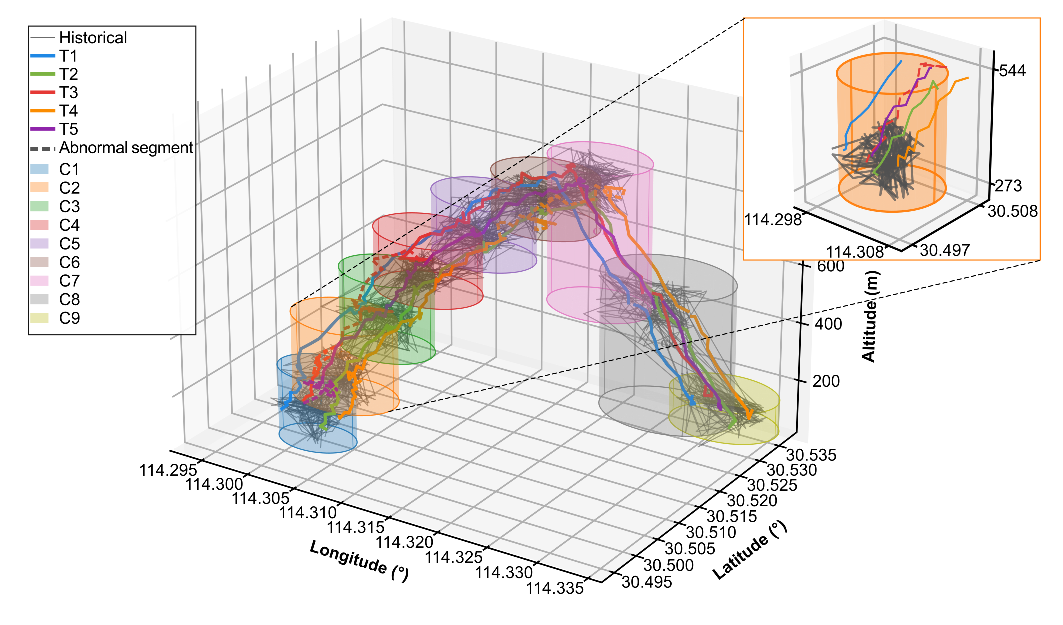
\includegraphics[width=\textwidth]{Fig2.eps}
  \caption{3D visualization of context sets and phase-specific trajectories anomaly detection}
    \label{fig:context_visualization}
\end{figure*}

\subsection{Parameter Sensitivity Analysis}

To examine robustness, we conduct a one-factor sensitivity analysis on three representative hyperparameters: the context-set memory slots $m$, the soft-assignment temperature $\tau$, and the hidden dimension $d_{model}$.
These parameters determine the capacity of peer-context representation, the sharpness of context discrimination, and the capacity of feature encoding, respectively.
The default configuration uses $m=8$, $\tau=1.0$, and $d_{model}=512$.
For each parameter, we vary its value while keeping all other settings unchanged as listed in Table~\ref{tab:hyperparameters}, and evaluate the resulting model on the SJ-SA-D1 dataset.
Each configuration is evaluated using five independent runs, and all values are reported as mean$\pm$standard deviation.
The corresponding one-factor results and trend comparisons are summarized in Table~\ref{tab:param_sensitivity}.

Overall, the repeated-run results indicate stable performance within a moderate hyperparameter range, whereas clearly under-capacitated settings cause consistent degradation.
For $m$, too few memory slots cannot cover the diversity of peer flight modes, while increasing the capacity beyond the main context patterns yields diminishing returns.
This suggests that the benefit of context-set memory depends more on adequate coverage than on maximizing the number of memory slots.
For $\tau$, an overly sharp assignment can fragment context discrimination, whereas an overly smooth assignment weakens the distinction between related and unrelated contexts.
The default temperature therefore provides a conservative balance between selectivity and stability.
For $d_{model}$, increasing the representation capacity improves performance when the model is under-parameterized, but further enlargement provides only marginal gains relative to the additional computational cost.
Taken together, the adopted settings offer a stable and practical compromise between detection performance, context coverage, and model complexity.

\subsection{Visualization Analysis}

To provide an intuitive understanding of the anomaly perception capability of CAFAD, we conduct qualitative visualization analyses from the perspectives of context-set distribution, phase-level anomaly localization, and feature representation on the SJ-SA-D1 dataset.

Fig.~\ref{fig:context_visualization} illustrates the constructed context sets and representative test trajectories in the three-dimensional flight space. 
The translucent cylinders denote different context sets from C1 to C9, while the gray curves represent historical trajectories. 
The colored curves from T1 to T5 correspond to several typical trajectories which share the same context sets, and the dashed segments indicate the detected abnormal flight phases. 
It can be observed that most normal trajectory segments evolve smoothly across adjacent context sets and remain consistent with the historical flight patterns. 
In contrast, abnormal segments exhibit noticeable deviations from the corresponding context distributions in specific flight phases. 
The zoom-in view further reveals the internal structure of a representative context set, demonstrating that CAFAD can identify local behavioral deviations at the phase-segment level rather than only producing trajectory-level anomaly decisions.

\begin{figure}[t]
\centering
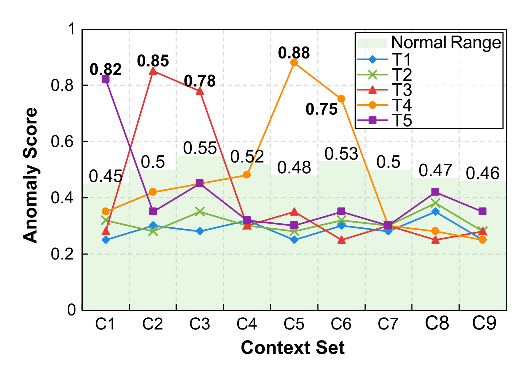
\includegraphics[width=\linewidth]{Fig3.eps}
\caption{Anomaly-score profiles}
\label{fig:score_visualization}
\end{figure}
To further analyze the detection behavior, Fig.~\ref{fig:score_visualization} presents the anomaly scores of representative trajectories across different context sets. 
In the relatively normal context sets C4, C7, C8, and C9, the scores of most trajectories stay below the corresponding normal range, typically around 0.25--0.38, which indicates stable context-consistent behavior. 
By contrast, clear score surges appear in several context-specific cases: T3 rises sharply in C2 and C3, T4 becomes prominent in C5 and C6, and T5 shows an obvious spike in C1, with these values exceeding the normal range by a noticeable margin. 
\begin{figure}[t]
\centering
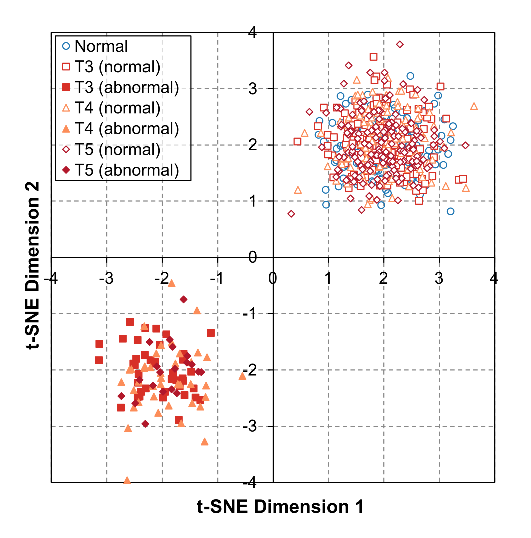
\includegraphics[width=\linewidth]{Fig4.eps}
\caption{Feature-space separation}
\label{fig:feature_visualization}
\end{figure}
This pattern suggests that CAFAD does not assign uniformly high scores to all trajectories, but instead highlights segments that deviate from the matched context set while keeping genuinely normal segments suppressed. 
Furthermore, the t-SNE visualization in Fig.~\ref{fig:feature_visualization} shows that normal and abnormal phase segments form distinguishable clusters with limited overlap in the learned feature space. 
This indicates that the proposed context-aware modeling and cross-perception attention mechanism can effectively capture the intrinsic differences between normal and abnormal flight behaviors.

\section{Conclusion}\label{sec:conclusion}
In this paper, we proposed CAFAD, a context-aware flight trajectory anomaly detection framework that jointly models phase-specific operational contexts and trajectory evolution patterns. 
CAFAD models phase-specific context sets and uses cross-perception attention to localize anomalous phase segments.
On the five SJ-SA sub-datasets, CAFAD achieves the highest F1 and generally the highest Recall, whereas 1D CNN-LSTM performs better on UMN-UAV.
Visualization results further show that CAFAD identifies local deviations from normal context distributions.
The results also suggest that its effectiveness depends on the diversity and phase structure of the trajectory data.

The evaluation is based on five repeated runs under a fixed trajectory-level split, so broader validation across additional datasets and split strategies remains necessary.
Future work will investigate semi-supervised learning strategies to reduce the dependence on labeled data and explore online adaptation mechanisms for handling continuously evolving flight environments.

\appendix
\section*{Appendix 1: Statistical results}
Tables~\ref{tab:appendix_f1_ci} and \ref{tab:appendix_sig} report the statistical results for the repeated-run experiments.
Table~\ref{tab:appendix_f1_ci} summarizes the 95\% confidence intervals for F1.
Table~\ref{tab:appendix_sig} reports paired $t$-test $p$-values and Hedges' $g$ effect sizes (small-sample corrected effect size).
Tables~\ref{tab:appendix_ablation_ci} and \ref{tab:appendix_ablation_sig} report the corresponding F1 confidence intervals, paired $t$-test $p$-values, and Hedges' $g$ effect sizes for the ablation study.
For SJ-SA-D1, we additionally checked the exact paired permutation test; due to $n=5$, the two-sided permutation $p$-value is highly discrete (step size $1/32=0.03125$, with many comparisons at $0.0625$), so we report paired $t$-test $p$-values as the primary inferential result and use Hedges' $g$ for effect magnitude.

\begin{table*}[!t]
\centering
\caption{95\% confidence intervals for F1 on the six datasets}
\label{tab:appendix_f1_ci}
\setlength{\tabcolsep}{0pt}
\renewcommand{\arraystretch}{1.0}
\tablebodyfont
\begin{tabularx}{\textwidth}{@{}l*{7}{>{\centering\arraybackslash}X}@{}}
\toprule
Dataset & TimesNet & TimeMixer & TSMixer & LSTM & \mbox{1D CNN-LSTM} & CTranATD & CAFAD \\
\midrule
SJ-SA-D1 & [0.8385, 0.8769] & [0.8313, 0.8695] & [0.8330, 0.8792] & [0.7952, 0.8084] & [0.8263, 0.8747] & [0.8527, 0.9081] & [0.9205, 0.9350] \\
SJ-SA-D2 & [0.7625, 0.7679] & [0.7470, 0.7606] & [0.7386, 0.7634] & [0.7804, 0.7872] & [0.8129, 0.8283] & [0.8266, 0.8424] & [0.9009, 0.9182] \\
SJ-SA-D3 & [0.7529, 0.7677] & [0.7309, 0.7416] & [0.7427, 0.7561] & [0.7917, 0.8024] & [0.8411, 0.8456] & [0.8492, 0.8559] & [0.8869, 0.9028] \\
SJ-SA-D4 & [0.7613, 0.7807] & [0.7652, 0.7712] & [0.7622, 0.7727] & [0.7817, 0.7892] & [0.8585, 0.8686] & [0.9146, 0.9200] & [0.9253, 0.9367] \\
SJ-SA-D5 & [0.7757, 0.7860] & [0.7365, 0.7600] & [0.7645, 0.7758] & [0.7881, 0.7957] & [0.8386, 0.8489] & [0.8473, 0.8580] & [0.9009, 0.9050] \\
UMN-UAV & [0.6568, 0.6676] & [0.7590, 0.7698] & [0.7458, 0.7535] & [0.8151, 0.8305] & [0.9055, 0.9141] & [0.6246, 0.6429] & [0.8780, 0.8925] \\
\bottomrule
\end{tabularx}
\end{table*}

\begin{table*}[!t]
\centering
\caption{Paired $t$-test $p$-values and Hedges' $g$ for CAFAD versus baseline methods on the six datasets}
\label{tab:appendix_sig}
\setlength{\tabcolsep}{2.5pt}
\renewcommand{\arraystretch}{1.0}
\tablebodyfont
\begin{tabularx}{\textwidth}{l*{6}{>{\centering\arraybackslash}X}}
\toprule
Dataset & TimesNet & TimeMixer & TSMixer & LSTM & \mbox{1D CNN-LSTM} & CTranATD \\
\midrule
SJ-SA-D1 & \pgcell{0.0005}{3.7222} & \pgcell{0.0003}{4.0924} & \pgcell{0.0009}{3.1716} & \pgcelllt{16.6919} & \pgcell{0.0006}{3.4603} & \pgcell{0.0060}{1.9057} \\
\midrule
SJ-SA-D2 & \pgcelllt{13.5350} & \pgcelllt{29.8828} & \pgcelllt{19.1704} & \pgcelllt{11.5451} & \pgcelllt{8.4760} & \pgcelllt{13.5919} \\
\midrule
SJ-SA-D3 & \pgcelllt{12.5360} & \pgcelllt{24.4113} & \pgcelllt{10.1925} & \pgcelllt{20.3272} & \pgcelllt{6.4442} & \pgcell{0.0001}{5.4358} \\
\midrule
SJ-SA-D4 & \pgcelllt{11.4361} & \pgcelllt{21.3122} & \pgcelllt{33.1003} & \pgcelllt{33.1722} & \pgcelllt{12.6894} & \pgcell{0.0017}{2.6867} \\
\midrule
SJ-SA-D5 & \pgcelllt{34.2804} & \pgcelllt{14.1361} & \pgcelllt{19.6421} & \pgcelllt{19.3534} & \pgcelllt{8.4628} & \pgcelllt{7.7434} \\
\midrule
UMN-UAV & \pgcelllt{26.6047} & \pgcelllt{18.0261} & \pgcelllt{21.9578} & \pgcelllt{9.6820} & \pgcell{0.0033}{-2.2407} & \pgcelllt{17.7488} \\
\bottomrule
\end{tabularx}
\end{table*}

\begin{table}[t]
\centering
\caption{95\% confidence intervals for the ablation study on SJ-SA-D1}
\label{tab:appendix_ablation_ci}
\setlength{\tabcolsep}{2.5pt}
\renewcommand{\arraystretch}{1.0}
\tablebodyfont
\begin{tabularx}{\columnwidth}{@{}l>{\centering\arraybackslash}X@{}}
\toprule
Configuration & 95\% CI \\
\midrule
Proposed Method & [0.9205, 0.9350] \\
w/o Context Set Memory & [0.8909, 0.9173] \\
w/o Cross-Attention & [0.8608, 0.8923] \\
w/o Time-Aware PE & [0.9163, 0.9296] \\
w/ Vanilla Attention & [0.8840, 0.9123] \\
\bottomrule
\end{tabularx}
\end{table}

\begin{table}[t]
\centering
\caption{Paired $t$-test $p$-values and Hedges' $g$ for F1 of CAFAD versus each variant on SJ-SA-D1}
\label{tab:appendix_ablation_sig}
\setlength{\tabcolsep}{3pt}
\renewcommand{\arraystretch}{1.0}
\tablebodyfont
\begin{tabularx}{\columnwidth}{@{}l*{2}{>{\centering\arraybackslash}X}@{}}
\toprule
Configuration & $p$-value & Hedges' $g$ \\
\midrule
w/o Context Set Memory & 0.0047 & 2.2048 \\
w/o Cross-Attention & 0.0005 & 4.1420 \\
w/o Time-Aware PE & 0.0659 & 0.6847 \\
w/ Vanilla Attention & 0.0038 & 2.6182 \\
\bottomrule
\end{tabularx}
\end{table}

\backmatter

\section*{Acknowledgements}

Not applicable.

\section*{Statements and Declarations}

\noindent\textbf{Funding.} This work was supported by the National Natural Science Foundation of China (Grant No. 62373094).

\medskip
\noindent\textbf{Competing interests.} The authors declare that there is no conflict of interest regarding the publication of this article.

\medskip
\noindent\textbf{Author contributions.} X.W. conceived the study, developed the methodology, and drafted the manuscript. 
Y.G. drafted and reviewed the manuscript, contributed to data preprocessing and model implementation. 
K.L. contributed to the experiments and data analysis. 
Z.L. provided critical feedback on the model design and analysis. 
X.Z. and W.Z. provided critical feedback on the model design. 
All authors reviewed and approved the final manuscript.

\medskip
\noindent\textbf{Data availability.} The SJ-SA dataset used in this study is publicly available at \url{https://github.com/cydhu/data/tree/master}. The UMN-UAV dataset is available from the University of Minnesota Digital Conservancy~\cite{umn_uav_dataset}.

\bibliography{sn-bibliography}

\end{document}
